%%%%%%%%%%%%%%%%%%%%%%%%%%%%%%%
%
%  Center for Environmental Genomics
%  Copyright (C) 2012 University of Washington.
%
%  Authors:
%  Vaughn Iverson  (vsi@uw.edu)
%  Chris Berthiaume (chrisbee@uw.edu)
%
% 
% This file is part of SEAStAR.
% 
% SEAStAR is free software: you can redistribute it and/or modify
% it under the terms of the GNU General Public License as published by
% the Free Software Foundation, either version 3 of the License, or
% (at your option) any later version.
% 
% SEAStAR is distributed in the hope that it will be useful,
% but WITHOUT ANY WARRANTY; without even the implied warranty of
% MERCHANTABILITY or FITNESS FOR A PARTICULAR PURPOSE.  See the
% GNU General Public License for more details.
% 
% You should have received a copy of the GNU General Public License
% along with SEAStAR.  If not, see <http://www.gnu.org/licenses/>.
%
%%%%%%%%%%%%%%%%%%%%%%%%%%%%%%% 

%%
\documentclass[10pt]{article}
\usepackage{geometry} % see geometry.pdf on how to lay out the page. There's lots.
\geometry{letterpaper} % or letter or a5paper or ... etc

\title{SEAS\lowercase{T}AR tools User Guide, version 0.3.0}
\author{Vaughn Iverson, Chris Berthiaume\\*\\*Armbrust Lab\footnote{http://armbrustlab.ocean.washington.edu}\\*School of Oceanography\\*University of Washington}

\usepackage{amsmath}
\usepackage{graphicx}
 
%%% BEGIN DOCUMENT
\begin{document}

\maketitle
\tableofcontents
\begin{center}
\line(1,0){250}
\end{center}
\section{Introduction}
The SEAStAR tools are a collection of programs which implement many data and processing intensive steps in an analysis pipeline producing quantitative analysis of alignments to reference databases, and/or binned assembled genomic scaffolds, directly from raw metagenomic next-generation sequence reads. (Figure \ref{fig:pipeline}). \subsection{Philosophy and limitations}
SEAStAR used to be an acronym for \underline{S}elect and \underline{E}stimate \underline{A}bundance from \underline{S}hor\underline{t} \underline{A}ligned \underline{R}eads. However, the set of tools and their capabilities have expanded well beyond that description, and so now SEAStAR is just the name of our whole analysis pipeline.

Our philosophy has been to create stable, modular, high-performance tools that fill important gaps we encountered between other established pre-existing tools in our pipeline. As such, you will see references to other packages in Figure \ref{fig:pipeline} and throughout this document.  We recognize that considerable innovation is ongoing in analysis software for next generation sequence, and so we have maintained a modular, pipelined approach to permit experimentation with, and substitution of, new tools as they become available.  Due to the wide variety of different computational environments that undoubtedly exist in different labs and institutes, our focus will be on releasing stable, documented, portable and high performance \emph{components} from our analysis pipeline, but not the pipeline scripts themselves.  This is because these scripts will need to be highly customized for both the goals and computational environment of any specific project.

Initially our goal is to release tools to enable others to work directly with datasets generated by the ABI SOLiD\texttrademark sequencing platform.  We recognize that some of the components we have developed may be valuable for use with Illumina\textsuperscript{\textregistered} sequence data, or with a mixture of sequence data types, but we will be placing the highest priority on completing our support for SOLiD data before evaluating which components in our pipeline are good candidates for generalizing to support both colorspace and nucleotide reads (see section \ref{sec:FASTQ} for more discussion of SOLiD data).  
   
\begin{figure}[p] % "placement and width parameter for the width of the image space.
\centering
\caption{Software pipeline diagram showing the planned release phases for the SEAStAR software.}
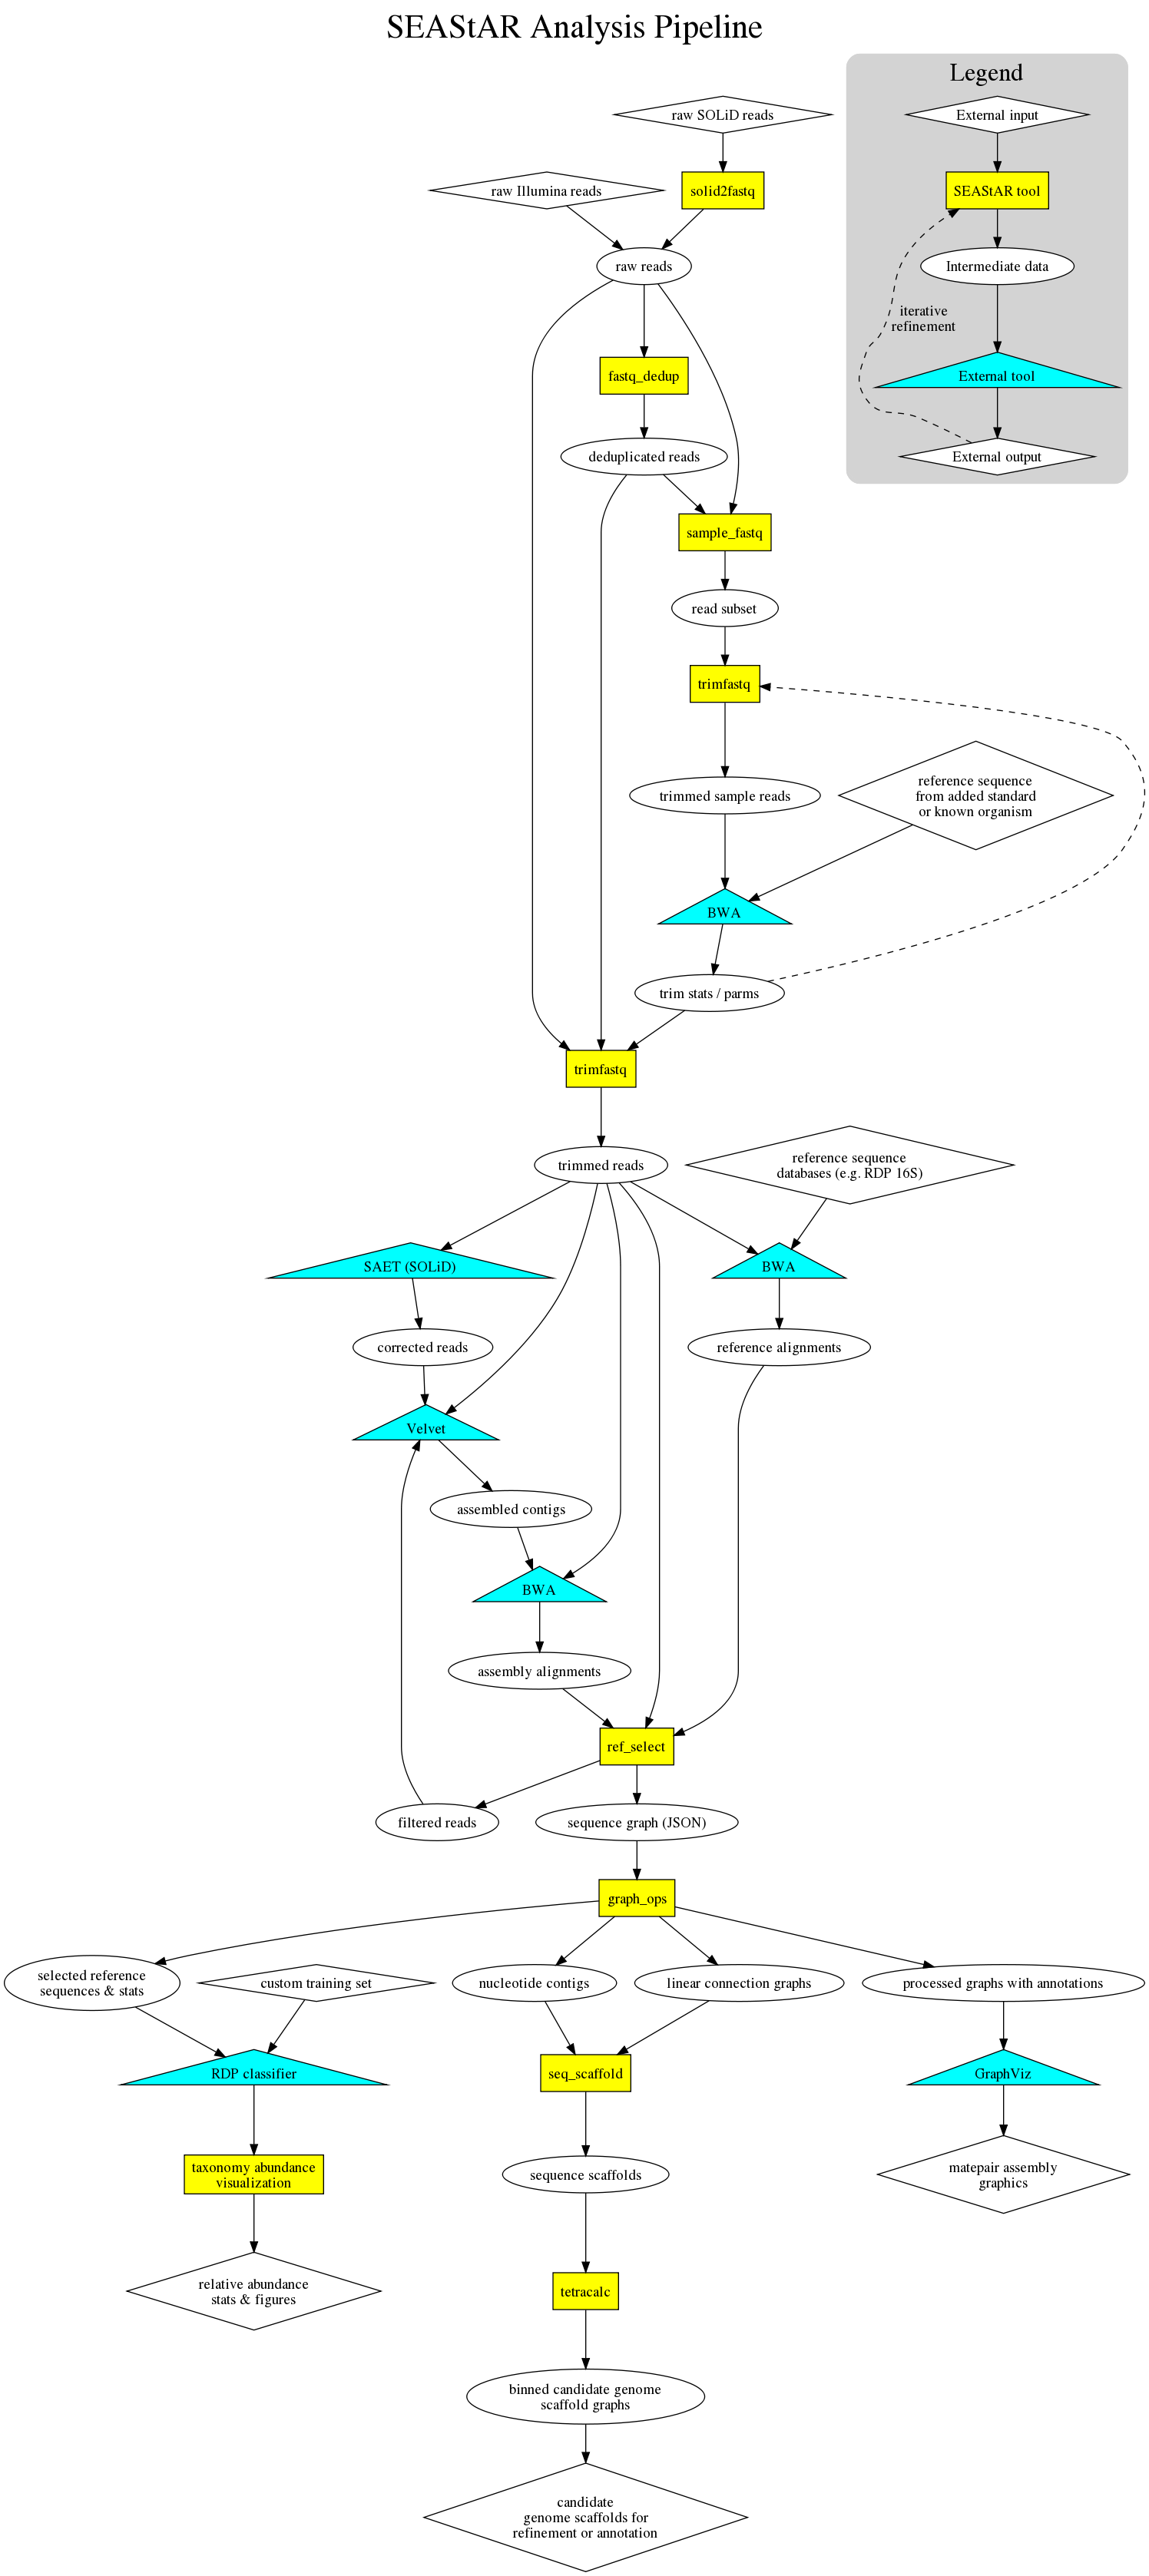
\includegraphics[height=\textheight]{SEAStAR_Pipeline_Stages.pdf}
\label{fig:pipeline}
\end{figure}
\subsection{Planned release phases}
The SEAStAR analysis pipeline is being released in three stages (Figure \ref{fig:pipeline}).  For up-to-date status information about the development and release process, please visit the SEAStAR website\footnote{http://armbrustlab.ocean.washington.edu/seastar}.

\begin{description}
\item[Stage 1 (current):]
Contains the tools we have developed for working with SOLiD� reads, converting them to colorspace FASTQ files, removing PCR duplicates, and trimming the reads based on quality and information content for various uses. Optional read error correction is performed by the SAET tool (a component of the denovo2 package\footnote{http://solidsoftwaretools.com/gf/project/denovo/frs/}). This code will enable the user to produce files that can be directly used with the BWA and Velvet packages for colorspace alignment and assembly, respectively.

\item[Stage 2 (future):]
Contains tools for processing SAM\footnote{http://samtools.sourceforge.net/} alignment files and assembled colorspace contigs into mate-paired assembly graphs with associated nucleotide contigs that can then be visualized and explored using GraphViz\footnote{http://www.graphviz.org/}. This stage's tools will also enable selection and visualization the best sequences from a reference database (e.g. the RDP\footnote{http://rdp.cme.msu.edu/} 16S database) alignment with associated statistics such as coverage and relative abundance. In the case of alignments with RDP, these sequences can then be classified (using the RDP classifier\footnote{http://sourceforge.net/projects/rdp-classifier/}) and visualized taxonomically.

\item[Stage 3 (future):]
Contains tools for splitting assembly graphs into parsimonious linear scaffold graphs, binning these scaffold graphs using tetra-nucleotide statistics, and constructing scaffold sequences with the order and orientation of contigs properly determined. Use of stage 3 tools enables production of candidate genome assemblies ready for refinement, gap-filling (if desired) and annotation. 
\end{description}

\subsection{Technical advice}
The next-generation sequence datasets that the SEAStAR tools are designed to work with are very large ($>$ one billion reads).  All compiled components of the SEAStAR tools are threaded and optimized for modern multi-core processors.  Many SEAStAR tools will take advantage of 8 or more cores, particularly when compressed (gzip format) input and output files are being processed.  When running on such a system, you will find that these components may run considerably more than 10$\times$ faster than equivalent tools written in a scripting language such as Perl or Python.  For this reason, the operation of such tools will often be "I/O bound"; that is: the performance bottleneck is the speed of the disk(s) and/or network connections connected to the workstation, and not the availability of CPU cycles.  The use of compressed files and local, independent disks for input and output files can often relieve some of this bottleneck and further improve run times.

Several of the SEAStAR tools---as well as many third-party tools used in our pipeline---have very high memory requirements when working with typical next-generation sequence datasets.  We note these cases in the discussion of each individual SEAStAR tool, and provide guidance about the impact different parameters will have on memory use.  However, in general, doing this kind of work will require a workstation with at least 64 gigabytes of DRAM, and depending on the dataset and the types of analysis your project requires, you may require some multiple of that amount (128, 256, or 512 gigabytes) to successfully implement an analysis pipeline that meets your needs.  In any case, when running these tools, it is highly advisable to set a session limit on the memory a process can attempt to allocate, to prevent machines from crashing and impacting other users who may be logged in.  For example, adding the Unix shell command:
\begin{verbatim}
      ulimit -v 64000000
\end{verbatim}
to any script that invokes high memory tools will effectively prevent a 64GB machine from being unintentionally brought down (i.e. thrashing the swap file) by an application that attempts to allocate more memory than is physically available.
\subsection{License and citation}
The SEAStAR tools are ``open source'' and are currently publicly distributed under the GPL version 3 license\footnote{http://gplv3.fsf.org/}.  Please contact the authors if you are interested in negotiating an alternative licensing arrangement.

We are in the process of preparing several publications specific to the SEAStAR analysis pipeline and the custom tools it contains.  In the interim, we ask that you cite the following paper (which was the first to use and describe these tools):\\*

\hangindent=1cm
\footnotesize{Iverson, V., Morris, R. M., Frazar, C. D., Berthiaume, C. T., Morales, R. L .and Armbrust, E. V., Untangling Genomes from Metagenomes: Revealing an Uncultured Class of Marine Euryarchaeota, \emph{Science} \textbf{335} pp.587-590 (2012)}
\normalsize
\section{Quick Start}
This section is a quick introduction to using SEAStAR tools for common use cases.  For installation instructions see the \verb+README+ file in the SEAStAR source tree.  Data used in these examples can be found in the \verb+test_data+ directory of the SEAStAR source tree.  Copy the following files from that directory to a new working directory.
\begin{verbatim}
        test_data/lambda_reads_F3.csfasta.gz
        test_data/lambda_reads_F3_QV.qual.gz
        test_data/lambda_reads_R3.csfasta.gz
        test_data/lambda_reads_R3_QV.qual.gz
        test_data/lambda.fasta.gz
\end{verbatim}
\subsection{Read preparation}
Convert SOLiD \verb+.csfasta+ and \verb+.qual+ files to gzipped \verb+.fastq+ files (see Section \ref{sec:FASTQ} for FASTQ format details).
\begin{verbatim}
solid2fastq -z lambda_reads lambda_conv
\end{verbatim}
Remove presumed PCR duplicate reads, identified by mate-pairs seen more than once.
\begin{verbatim}
fastq_nodup -z -l 13 -d 2 -e 3 lambda_conv lambda_dedup
\end{verbatim}
Trim and filter the de-duplicated FASTQ reads based on read quality, information content, and length.
\begin{verbatim}
trimfastq -z -p 0.5 -l 34 -m 34 -e 3.0 --add_len lambda_dedup lambda_trim
\end{verbatim}
Randomly sample reads from \verb+.fastq+ files, retaining approximately 10\% of the original reads.  Randomly subsampled read sets are useful for quickly tuning the parameters of \verb+trimfastq+ for a given set of reads against some reference.
\begin{verbatim}
samplefastq -z -f 0.1 lambda_trim lambda_trim_samp
\end{verbatim}
\subsection{Alignment to a reference}
If the short read aligner BWA\footnote{Available from: http://bio-bwa.sourceforge.net/} (version $\le$ 0.5.10) is installed it can be used to align de-duplicated and trimmed lambda FASTQ reads against the lambda reference genome.  The resulting alignment file is in SAM format.
\begin{verbatim}
bwa index -a is -c lambda.fasta.gz

bwa aln -c -n 0.001 -l 18 lambda.fasta.gz lambda_trim.read1.fastq.gz 
     >lambda_trim.read1.sai

bwa samse -n 1000000 lambda.fasta.gz lambda_trim.read1.sai 
     lambda_trim.read1.fastq.gz 2>lambda_trim.read1.samse.log 
     >lambda_trim.read1.sam

bwa aln -c -n 0.001 -l 18 lambda.fasta.gz lambda_trim.read2.fastq.gz 
     >lambda_trim.read2.sai

bwa samse -n 1000000 lambda.fasta.gz lambda_trim.read2.sai 
     lambda_trim.read2.fastq.gz 2>lambda_trim.read2.samse.log 
     >lambda_trim.read2.sam

bwa aln -c -n 0.001 -l 18 lambda.fasta.gz lambda_trim.single.fastq.gz 
     >lambda_trim.single.sai

bwa samse -n 1000000 lambda.fasta.gz lambda_trim.single.sai 
     lambda_trim.single.fastq.gz 2>lambda_trim.single.samse.log 
     >lambda_trim.single.sam
\end{verbatim}
\subsection{De novo assembly}
If the colorspace aware build of the de novo assembly tool Velvet\footnote{Available from: http://www.ebi.ac.uk/$\sim$zerbino/velvet/} is installed it can be used to assemble lambda colorspace contigs.  First re-trim reads at a stricter quality cutoff and output a Velvet style \verb+.fastq+ file of interleaved mate-pairs, then assemble with Velvet.
\begin{verbatim}
trimfastq -z --mates_file -p 0.9 -l 34 -m 34 --add_len -e 3.0 lambda_dedup 
     lambda_trimvelvet

velveth_de lambda_asm/ 15 -fastq.gz -shortPaired lambda_trimvelvet.mates.fastq.gz 
     -short lambda_trimvelvet.single.fastq.gz >lambda_asm.velveth_de.log 2>&1

velvetg_de lambda_asm/ -scaffolding no -read_trkg no -ins_length auto 
     -ins_length_sd auto -exp_cov 50 -cov_cutoff 5 -min_contig_lgth 50 
     >lambda_asm.velvetg_de.log 2>&1
\end{verbatim}
\section{Command Reference}
\subsection{solid2fastq}

This tool converts SOLiD \verb+.csfasta+ and \verb+.qual+ input files (raw reads transferred off the instrument) to output files that are an interoperable variant of the FASTQ file format (see SEAStAR FASTQ format details in section \ref{sec:FASTQ}).
\\*
\\*
Usage:   \verb+solid2fastq [options] <in_prefix> <out_prefix>+
\\*
\\*
Where \verb+<in_prefix>+  denotes the input prefix which is the part of the input filename shared in common between all \verb+.csfasta+ and \verb+.qual+ files generated by the same sequence library. It is typically shown in the \verb+Title:+ comment line near the top of \verb+.csfasta+ format input files.  For example: 
\begin{verbatim}
        # Title: GG050409_20090604_matepair_50
\end{verbatim}
is found near the top of input files:
\begin{verbatim}
        GG050409_20090604_matepair_50_R3.csfasta
        GG050409_20090604_matepair_50_R3_QV.qual
        GG050409_20090604_matepair_50_F3.csfasta
        GG050409_20090604_matepair_50_F3_QV.qual
\end{verbatim}
And so use of \verb+GG050409_20090604_matepair_50+ for \verb+<in_prefix>+ will specify these four files for input to the \verb+solid2fastq+ tool.

Note that \verb+solid2fastq+ relies on the SOLiD naming conventions for the suffixes of these files (e.g. \verb+_R3.csfasta+).  You are free to rename these files with different prefixes, but the suffixes must remain the same.  You may, however, compress these files using gzip and add the customary \verb+.gz+ suffix at the very end of the filename, which tells \verb+solid2fastq+ to decompress the files as it reads them.

The \verb+<out_prefix>+ parameter is similar to the \verb+<in_prefix>+ as it is used to name the output \verb+.fastq+ file(s) generated by this tool.  The output prefix may be any text, except you should generally avoid whitespace and punctuation characters other than ``\verb+_+''.  This is because, by default, the names of all output reads are also prefixed with this string and the variant of the FASTQ format used by the SEAStAR tools depends on certain punctuation characters to quickly parse these read names (see SEAStAR FASTQ format in section \ref{sec:FASTQ} for details).  This file naming constraint may be relaxed through the use of optional parameters described below.

Note that \verb+<in_prefix>+ and/or \verb+<out_prefix>+ may contain directory path information, but in the case of \verb+<out_prefix>+ this will necessitate the use of the \verb+--prefix+ or \verb+--no_prefix+ options (described below).

\verb+solid2fastq+ writes a single output \verb+.fastq+ file for each matching pair of \verb+.csfasta+ / \verb+.qual+ input files.  The names of these output files are constructed as:
\\*\\*
\verb+        <in_prefix>_F3[.csfasta|_QV.qual]+ $\to$ \verb+<out_prefix>.read1.fastq+\\*
\verb+        <in_prefix>_R3[.csfasta|_QV.qual]+ $\to$ \verb+<out_prefix>.read2.fastq+\\*\\*
\verb+        +singlets from \verb+F3/R3+ $\to$ \verb+<out_prefix>.single.fastq+
\\*\\*
Note that for paired-end libraries, alternate naming suffix conventions for the \verb+R3+ input are also recognized (substituting \verb+F5-BC+ or \verb+F5-P2+ for \verb+R3+). 

Additionally, for paired libraries (mate-paired or paired-end) should \verb+solid2fastq+ encounter any singlet reads (those with a missing mate), they are by default given the appropriate suffix and then written to a file named: 
\begin{verbatim}
        <out_prefix>.single.fastq
\end{verbatim}
\verb+solid2fastq+ optional parameters \verb+[options]+:
\begin{verbatim}
        [-h|--help] [--version] [--prefix=<string>] [-n|--no_prefix]
        [-z|--gzip] [-b|--bc=<BC>] [-s|--singles]
\end{verbatim}
\begin{verbatim}
-h
--help
\end{verbatim}
Print a guide to valid command line parameters and their correct usage to the terminal, and then exit.

\begin{verbatim}
--version
\end{verbatim}
Print the version number of the executing program and then exit.

\begin{verbatim}
--prefix=<string>    
\end{verbatim}
Specify the prefix string to add to read identifiers.  For example, \verb+.csfasta+ read identifier:
\begin{verbatim}
        >1_68_381_F3
\end{verbatim}
will become:
\begin{verbatim}
        @xx+<string>:1_68_381/1
\end{verbatim}
in the \verb+.fastq+ output file.  By default this is \verb+<out_prefix>+ described above. 

The use of a terse, but unique, prefix string is advisable because it helps identify the source, and processing steps, performed on a set of reads as they flow through an analysis pipeline. Keep in mind that this text will be added to the output file for every read, so short strings are preferable. The output prefix may be any text you would like, except you may not use whitespace or punctuation characters other than ``\verb+_+''.
\begin{verbatim}
-n
--no_prefix 
\end{verbatim}
Overrides the default read prefixing behavior and instead preserves the read identifiers as they are in the input \verb+.csfasta+ file(s).  For example:
\begin{verbatim}
        >1_68_381_F3
\end{verbatim}
simply becomes:
\begin{verbatim}
        @xx+:1_68_381/1
\end{verbatim}
\begin{verbatim}
-z
--gzip
\end{verbatim}
Write output \verb+.fastq+ files compressed in the gzip format, and with filenames suffixed \verb+.gz+.

\begin{verbatim}
-b <BC>
--bc=<BC>
\end{verbatim}
Used only for barcoded SOLiD libraries, in addition to \verb+<in_prefix>+, to specify input files for a specific barcode (\verb+<BC>+).

\begin{verbatim}
-s
--singles             
\end{verbatim}
Write two separate singlet files that segregate the singlets by input files.  This is useful for doing strand-specific analyses using paired-end libraries, where the mated reads are sequenced from opposite strands.  For example:
\\*\\*
\verb+        <in_prefix>_F3[.csfasta|_QV.qual]+ $\to$ \verb+<out_prefix>.read1.fastq+\\*
\verb+        +singlets from \verb+F3+ $\to$ \verb+<out_prefix>.single1.fastq+
\\*\\*
\verb+        <in_prefix>_R3[.csfasta|_QV.qual]+ $\to$ \verb+<out_prefix>.read2.fastq+\\*
\verb+        +singlets from \verb+R3+ $\to$ \verb+<out_prefix>.single2.fastq+

\subsection{fastq\_nodup}

This tool reads paired \verb+.fastq+ files (with associated singlets), and removes the lowest quality pair(s) of presumed PCR duplicate reads.  This operation assumes that multiple read-pairs sharing substantially the same sequences for both mates are statistically unlikely to occur frequently at random (due to the distribution of insert sizes), and therefore represent likely artifactual duplications resulting from PCR over-amplification during library construction. If this assumption does not hold for a given library, then use of this tool is inappropriate. 

Notably, this tool is most appropriate for metagenomes---or any other sample type---where no reference genome is available for performing duplicate removal through reference alignments.  This is because \verb+fastq_nodup+ works entirely through error-tolerant internal comparisons of read-pairs to each other within an entire sequenced library.

To accomplish this, \verb+fastq_nodup+ builds a large table of sequence prefixes, requiring a substantial amount of memory.  The amount of memory required can be controlled through tuning the various parameters, but a minimum of 32Gb will probably be necessary for most read datasets.

Note that singlet reads are also randomly removed in the same proportion as matching mated reads.  This is done assuming that PCR duplicated pairs are as likely to produce singlets as non-duplicated pairs.  For example:
\\*\\*
\verb+        S1, S1, M1 -- M2, M1 -- M2, M1 -- M3+  
\\*\\*
In the above example \verb+S+=singlet reads, \verb+M+=mated reads, and the numeric suffixes indicate matching sequences.  So the lowest quality pair of \verb+M1--M2+ mates will be removed from the output, and each of the \verb+S1+ reads will have a $\tfrac{1}{3}$ probability of being removed (disregarding quality). The $\tfrac{1}{3}$ probability is calculated from the fact that $\tfrac{1}{3}$ of the pairs containing sequence \verb+M1+ were presumed PCR duplicates and therefore removed.
\\*
\\*
Usage:  \verb+fastq_nodup [options] <in_prefix> <out_prefix>+
\\*
\\*
where \verb+<in_prefix>+ and \verb+<out_prefix>+ specify the input and output filename prefixes to use for input files and naming output files.  For example:
\\*\\*
\verb+        <in_prefix>.read1.fastq+ $\to$ \verb+<out_prefix>.read1.fastq+\\*
\verb+        <in_prefix>.read2.fastq+ $\to$ \verb+<out_prefix>.read2.fastq+\\*
\verb+        <in_prefix>.single.fastq+ $\to$ \verb+<out_prefix>.single.fastq+
\\*\\*
The input files may be gzip format compressed files with the customary \verb+.gz+ suffix at the very end of the filename, which tells \verb+solid2fastq+ to decompress the files as it reads them. Multiple single files (i.e. \verb+.single1.fastq+ and \verb+.single2.fastq+ suffixes) are also recognized.
\\*
fastq\_nodup optional parameters \verb+[options]+:
\begin{verbatim}
        [-h|--help] [--version] [-v|--verbose] [-z|--gzip]
        [--prefix=<string>] [--no_prefix] [-l|--index_len=<u>]
        [-m|--match_len=<u>] [-d|--index_err=<u>] [-e|--match_err=<u>]
        [--seed=<n>]
\end{verbatim}
\begin{verbatim}
-h
--help
\end{verbatim}
Print a guide to valid command line parameters and their correct usage to the terminal, and then exit.

\begin{verbatim}
--version
\end{verbatim}
Print the version number of the executing program and then exit.

\begin{verbatim}
-v
--verbose
\end{verbatim}
Print additional statistics and diagnostic information about the run.

\begin{verbatim}
-z
--gzip
\end{verbatim}
Write output \verb+.fastq+ files compressed in the gzip format, and with filenames suffixed \verb+.gz+.

\begin{verbatim}
--prefix=<string>    
\end{verbatim}
Specify the prefix string to add to read identifiers.  For example:
\begin{verbatim}
        @xx+<string>:1_68_381/1
\end{verbatim}
Note, this will replace any existing prefix.  By default this is \verb+<out_prefix>+ described above.

\begin{verbatim}
-n
--no_prefix 
\end{verbatim}
Overrides the default read prefixing behavior and instead preserves the read identifiers exactly as they are in the input fastq file(s).

\begin{verbatim}
-l <u>
--index_len=<u>        
\end{verbatim}
Controls the read sequence prefix length of the search index.  This should be set long enough so that random prefix collisions are infrequent, but short enough so that a large number of sequence errors are unlikely to accumulate.  This parameter also impacts the memory use of this tool, with each increment increasing the index size by a factor of 4. This parameter defaults to \verb+<u>+=14 nucleotides and may not exceed 32 nucleotides.

Both mates of each read-pair are indexed, and this indexed look-up is used to find a list of mate sequences corresponding to each sequence prefix.  Given that the mates also must match, it is acceptable for a low-level of prefix collisions to occur in this index.  That is, assuming the level of prefix collision is low (only a small number of non-duplicated reads share any given prefix), it will be highly improbable that reads matching a given prefix will share mates with matching sequence at random.

\begin{verbatim}
-m <u>
--match_len=<u>
\end{verbatim}
Controls the required match length of the unindexed mate in detecting a duplicate pair.  Like the previous parameter (\verb+--index_len+), this setting has an impact on memory use, although memory requirements only increase linearly with match length.  This parameter should be set as high as memory permits to improve specificity.   

This parameter defaults to the full read length, although lower settings are acceptable assuming that the \verb+--index_len+ is appropriately set, and the sum of \verb+index_len+ and \verb+match_len+ exceeds about 35 nucleotides (that is, random 35 nucleotide joint index-match collisions are extremely unlikely assuming each match is sufficiently long).

\begin{verbatim}
-d <u>
--index_err=<u>     
\end{verbatim}
Controls the number of mismatches tolerated in the indexed sequence prefix while still permitting a sequence match.  This value defaults to \verb+<u>+=1 and may be set in the range 0--2.  This setting has a major impact on run time, with each increment increasing it by a factor of about 4.  Duplicated reads with more than \verb+index_err+ mismatches in the \verb+index_len+ prefix may still be found by the mate's indexed prefix, assuming that it does not also have more than \verb+index_err+ errors.  

\begin{verbatim}
-e <u>
--match_err=<u>   
\end{verbatim}
Controls the number of mismatches tolerated in a matched mate sequence (in the \verb+match_len+ prefix).  This value defaults to 3 and must be $\ge$ 0.  This setting has little impact on run time.  Setting \verb+match_err+ to higher values will reduce the specificity of the mate-matching and should therefore be accompanied by correspondingly larger values of \verb+match_len+.
\begin{verbatim}
--seed=<n>
\end{verbatim}
Integer seed used by the internal pseudo-random number generator. This only affects the random selection of matching singlets (as described above).  Defaults to \verb+<n>+=12345. 

\subsection{samplefastq}
This tool randomly samples reads from a given set of fastq files, producing a corresponding set of output fastq files.  This is useful for more quickly tuning parameters for the \verb+trimfastq+ tool (described below) and for producing simulated read datasets for various other purposes.  
\\*
\\*
Usage: \verb+samplefastq -f <float>|<int> [options] <in_prefix> <out_prefix>+
\\*
\\*
where the mandatory \verb+-f+ parameter indicates how the input files should be sampled and \verb+<in_prefix>+ and \verb+<out_prefix>+ specify the input and output filename prefixes to use for input files and naming output files.   For example:
\\*\\*
\verb+        <in_prefix>.read1.fastq+ $\to$ \verb+<out_prefix>.read1.fastq+\\*
\verb+        <in_prefix>.read2.fastq+ $\to$ \verb+<out_prefix>.read2.fastq+\\*
\verb+        <in_prefix>.single.fastq+ $\to$ \verb+<out_prefix>.single.fastq+
\\*\\*
The input files may be gzip format compressed files with the customary \verb+.gz+ suffix at the very end of the filename, which tells \verb+solid2fastq+ to decompress the files as it reads them. Multiple single files (i.e. \verb+.single1.fastq+ and \verb+.single2.fastq+ suffixes) are also recognized.

Note that for paired sequences (as shown above) read pairs are always sampled together; that is, each pair of reads counts at a single read unit for sampling purposes, as does each singlet read. 
\\*\\*
\verb+samplefastq+ manditory parameter \verb+-f+:
\\*\\*
\verb+-f <float>+ or \verb+<int>+\\*
\verb+--frac_sample=<float>+ or \verb+<int>+
\\*\\*
The \verb+-f+ parameter tells \verb+samplefastq+, either directly or indirectly, how many output reads to randomly sample from the input \verb+.fastq+ files.  Values $<$ 1.0 are interpreted as a fraction of the input reads to retain, whereas values $\ge$ 1.0 are rounded to an integer count of reads to retain.  

Note that when a read count is provided, the input files must be read twice by \verb+samplefastq+; once to count the number of input reads, and then again to randomly sample those reads. Once the number of input reads is known, the requested read count is converted into a fraction and operation proceeds as though that fraction had been initially provided to the \verb+-f+ parameter.  Therefore, if a given set of inputs is to be sampled repeated, it will be considerably more efficient to obtain the count of reads once and calculate the fraction to retain for each subsequent sampling.
The requested (or calculated) fraction of reads to sample is used internally as the probability of retaining each read (or pair) and each is considered an independent trial.  Because of this, the precise fraction (or count) of reads requested is unlikely to be generated, although the sampled output will typically be very close to that requested. 
\\*\\*
\verb+samplefastq+ optional parameters \verb+[options]+:
\begin{verbatim}
[-h|--help] [--version] [--seed=<int>] [-z|--gzip]
\end{verbatim}
\begin{verbatim}
-h
--help
\end{verbatim}
Print a guide to valid command line parameters and their correct usage to the terminal, and then exit.

\begin{verbatim}
--version
\end{verbatim}
Print the version number of the executing program and then exit.

\begin{verbatim}
-z
--gzip
\end{verbatim}
Write output fastq files compressed in the gzip format, and with filenames suffixed \verb+.gz+.

\begin{verbatim}
--seed=<n>
\end{verbatim}
Integer seed used by the internal pseudo-random number generator.  To obtain different samples from the same input file(s), set this parameter to different values.  Repeated runs with all parameters the same will produce identical outputs.  Defaults to \verb+<n>+=12345.

\subsection{trimfastq}

This tool is used to trim or reject individual reads on the basis of quality scores.  Reads may also be rejected based on low information content (entropy). When run on paired reads, this operation is performed on mates independently, and when one mate of a pair is rejected, the other becomes a singlet.

Trimming based on quality scores is performed with the goal of producing trimmed reads that have a calculated probability of error below some threshold.  That is, bases are trimmed off the 3' end of the read until the remaining bases have a joint probability of error below a threshold.  For example, if a threshold of 0.5 is selected, that means the output reads will be expected to have, on average, 0.5 erroneous nucleotides per read. 

For colorspace (SOLiD differentially encoded) reads, the probability of error is calculated as the joint probability of error in each of two consecutive color positions.  That is, because single color errors will typically be correctable, the probability of a nucleotide error at a given position is the probability that both corresponding color positions are erroneous (i.e. the pairwise product of color error probabilities yields the probability of uncorrectable nucleotide errors).

Minimum read lengths may also specified such that reads trimmed shorter than the specified minimum to meet an error probability threshold will instead be rejected.

Reads may also be independently rejected for failing to have a minimum mean information content.  \verb+trimfastq+ optionally calculates the mean entropy of each read (as average bits per dinucleotide) and reject reads that fail to meet a given threshold.  A common error for next-generation sequencers is to produce junk reads where all or part of the read contains highly repetitive (low information) sequence.  Random DNA sequence contains 4 bits per dinucleotide of entropy, and we have observed that (non-repeat) natural sequences typically contain more than 3 bits per dinucleotide.
\\*
\\*
Usage:  \verb+trimfastq [options] <in_prefix> <out_prefix>+
\\*
\\*
where \verb+<in_prefix>+ and \verb+<out_prefix>+ specify the input and output filename prefixes to use for input files and naming output files.  For example:
\\*\\*
\verb+        <in_prefix>.read1.fastq +$\to$ \verb+<out_prefix>.read1.fastq+\\*
\verb+        <in_prefix>.read2.fastq +$\to$ \verb+<out_prefix>.read2.fastq+\\*
\verb+        <in_prefix>.single.fastq +$\to$ \verb+<out_prefix>.single.fastq+
\\*\\*
The input files may be gzip format compressed files with the customary \verb+.gz+ suffix at the very end of the filename, which tells \verb+solid2fastq+ to decompress the files as it reads them. Multiple single files (i.e. \verb+.single1.fastq+ and \verb+.single2.fastq+ suffixes) are also recognized.
\\*\\*
\verb+trimfastq+ optional parameters \verb+[options]+:
\begin{verbatim}
        [-h|--help] [--version] [-c|--color_space] [-z|--gzip]
        [-v|--invert_singles] [-s|--singles]  [-p|--correct_prob=<d>]
        [-l|--min_read_len=<u>] [-m|--min_mate_len=<u>]
        [-f|--fixed_len=<u>] [--prefix=<string>] [--add_len]
        [--no_prefix] [-e|--entropy_filter=<d>] [--entropy_strict]
        [--mates_file]
\end{verbatim}
\begin{verbatim}
-h
--help
\end{verbatim}
Print a guide to valid command line parameters and their correct usage to the terminal, and then exit.

\begin{verbatim}
--version
\end{verbatim}
Print the version number of the executing program and then exit.

\begin{verbatim}
-z
--gzip
\end{verbatim}
Write output fastq files compressed in the gzip format, and with filenames suffixed \verb+.gz+.

\begin{verbatim}
--prefix=<string>    
\end{verbatim}
Specify the prefix string to add to read identifiers.  For example:
\begin{verbatim}
        @xx+<string>:1_68_381/1
\end{verbatim}
Note, this will replace any existing prefix.  By default this is  \verb+<out_prefix>+ described above.

\begin{verbatim}
-n
--no_prefix 
\end{verbatim}
Overrides the default read prefixing behavior and instead preserves the read identifiers exactly as they are in the input fastq file(s).

\begin{verbatim}
--add_len
\end{verbatim}
Add the final trimmed length value to the read prefix.  For example:
\begin{verbatim}
        @TT+lambda:1_81_912/1
        TGTTGTGCGCGCCATAGCGAGGGGCTCAGCACGCGTCCCTCCGCCCCAC
        +
        5/0)358)%57*)%881/(/4'.'53*&#91*-'&,&%$''%&'46-+#
\end{verbatim}
Trims to (where \verb+37+ in the first line indicates the final trimmed length) :
\begin{verbatim}
        @TT+37|lambda_trim:1_81_912/1
        TGTTGTGCGCGCCATAGCGAGGGGCTCAGCACGCGTC
        +
        5/0)358)%57*)%881/(/4'.'53*&#91*-'&,&
\end{verbatim}
\begin{verbatim}
-c
--color_space
\end{verbatim}
Use color-space errors to trim and reject reads.  This overrides the preferred default behavior of using uncorrectable nucleotide space errors for trimming colorspace reads.  However, for trimming non-colorspace reads (e.g. Illumina reads) this parameter should be used, as error correction through differential encoding is not possible with such reads.
\begin{verbatim}
-v
--invert_singles
\end{verbatim}
Causes singlet file(s) output to be the opposite configuration of the input.  That is:
\\*\\*
\verb+        <in_prefix>.single.fastq + $\to$ \verb+ <out_prefix>.single[12].fastq+
\\*
or
\\*
\verb+        <in_prefix>.single[12].fastq+ $\to$ \verb+ <out_prefix>.single.fastq+
\\*\\*
Note that this option is only valid when there are input singlet reads.

\begin{verbatim}
-s
--singles
\end{verbatim}
Write two singlet files (\verb+.single1.fastq+ and \verb+single2.fastq+), one for new singlets generated from each paired input file.   Note that this option is only valid when there are no input singlet reads.  The default behavior in this case is to write a single combined singlet file (\verb+.single.fastq+).

\begin{verbatim}
-p <d>
--correct_prob=<d>
\end{verbatim}
Minimum mean probability that trimmed output reads are free of uncorrectable errors (or all errors with \verb+-c+).  Default value is \verb+<d>+=0.5.

\begin{verbatim}
-l <u>
--min_read_len=<u>
\end{verbatim}
Minimum length of a singlet or longest-mate of a pair, in nucleotides. Default value is \verb+<u>+=24 bases.

\begin{verbatim}
-m <u>
--min_mate_len=<u>
\end{verbatim}
Minimum length of the shortest mate of a pair, in nucleotides.  Default value is the value provided for  \verb+--min_read_len+.  This value must be $\le$ the value used for  \verb+--min_read_len+.  Use of this parameter allows paired reads shorter than  \verb+min_read_len+ to be retained as long as their mate satisfies  \verb+min_read_len+.  
\begin{verbatim}
-f <u>
--fixed_len=<u>
\end{verbatim}
Trim all reads to a fixed length, still rejecting reads that don't meet specified quality thresholds at this length.  Default is no fixed length.
\begin{verbatim}
-e <d>
--entropy_filter=<d>
 \end{verbatim}

Reject reads with mean per position measured information (entropy) below the given value (in bits per dinucleotide).  The range of valid values is 0.0--4.0 inclusive.  By default this filter is off.

\begin{verbatim}
--entropy_strict
\end{verbatim}

Reject reads for low entropy overall, not just the retained part after trimming.  By default this setting is off.  Use of this setting requires use of  \verb+--entropy_filter+. 

\begin{verbatim}
--mates_file
\end{verbatim}
In addition to other outputs, produce a Velvet compatible mate-paired output file (named  \verb+<out_prefix>_mates.fastq+) with read2 mates reversed as required. 

\section{Colorspace FASTQ Format Reference}
\label{sec:FASTQ}

The SEAStAR tools use certain conventions for organizing read data in \verb+.fastq+ files.  This section describes these conventions in sufficient detail to understand the operation of the tools described in this document.

SOLiD reads and associated quality statistics from the instrument are packaged in FASTA-like format files called \verb+.csfasta+ and \verb+.qual+ files.  Fragment (non-paired) libraries produce a single matched set of files named by convention as:
\\*\\*
\verb+        <prefix>_F3.csfasta  +and \verb+ <prefix>_F3_QV.qual+ 
\\*\\*
Paired libraries (either mate-paired or paired-end) additionally produce a second matched set of files named:
\\*\\*
\verb+        <prefix>_R3.csfasta  +and \verb+ <prefix>_R3_QV.qual+ 
\\*\\*
For some paired-end libraries, the \verb+R3+ in these (second mate) files may be replaced by \verb+F5-BC+ or \verb+F5-P2+.  

There is no guarantee that every read in an \verb+F3+ file has a corresponding mate in an \verb+R3+ file, or vice-versa.  These unmated reads are called ``singlets''.

Most open source tools do not support these off-instrument SOLiD FASTA-like files, and so they must be converted to FASTQ format files for compatibility.  This is complicated by the fact that SOLiD reads do not represent nucleotides, but are instead differential encoded colorspace reads, where each numbered color represents a coded di-nucleotide transition\footnote{See SOLiD colorspace whitepaper for more details:\\http://www3.appliedbiosystems.com/cms/groups/mcb\_marketing/documents/generaldocuments/cms\_058265.pdf} (e.g. \verb+AA+ = \verb+0+, \verb+AC+ = \verb+1+, etc.).  For colorspace reads to be translated into nucleotide space, an initial known base, the primer base, is required.  The following example shows the colorspace sequence for one read prefixed with primer base ``\verb+T+'': 
\begin{verbatim}
        >1_68_381_F3
        T01200011211220011021332321220121211221111322011220
\end{verbatim}
One simple approach to using these reads would be to simply convert them to nucleotide space \verb+.fastq+ files and from that point onwards ignore the colorspace source of the reads.  Unfortunately, this does not work well because colorspace errors at any position in a read will effectively corrupt all of the resulting converted nucleotide sequence from the erroneous position(s) onwards.  In addition, there are distinct potential advantages to processing (aligning and assembling) SOLiD reads in colorspace, delaying conversion to nucleotide space until later in the analysis pipeline when it can be done much more accurately (due to the error correction potential of the di-nucleotide encoding).  For these reasons, the SEAStAR tools preserve the colorspace information in the FASTQ representation.

To accomplish this, we follow the convention used by MAQ, BWA and Velvet, mapping colorspace numbers to colorspace letters as \verb+[0123.]+ $\to$ \verb+[ACGTN]+.  Because the initial primer base and its following color value are not from the sampled DNA, and thus will not correspond to the actual sequence $\sim$75\% of the time, these two values need to be removed from the colorspace read data that is actually used for alignment or assembly.  However, they need to be kept in some form so that the original nucleotide sequence of the read can be reconstructed at a later stage in the pipeline.  To handle this, we have developed the following convention:
\\*\\*
Original colorspace \verb+.csfasta+ read:
\begin{verbatim}	
        >1_68_381_F3
        T012000112112200110213323212201212112211113220..2.0
\end{verbatim}
Convert to colorspace letters:	
\begin{verbatim}	
        >1_68_381_F3
        TACGAAACCGCCGGAACCAGCTTGTGCGGACGCGCCGGCCCCTGGANNGNA
\end{verbatim}
Convert to FASTQ format (with quality information added), relocating the primer base and following color ``\verb+TA+'' to the header line (discarding the initial quality value):
\begin{verbatim}
        @TA+lambda:1_68_381/1
        CGAAACCGCCGGAACCAGCTTGTGCGGACGCGCCGGCCCCTGGACCGGA
        +
        9'4,)9,*%4/'#,32)*.1-1(5&3,%,$:*&#'8,+2'40$)05(,&
\end{verbatim}
The read prefix \verb+lambda+ is added as an identifier for this set of reads, by default, from the \verb+.csfasta+ filename prefix.  The read name suffix changes from the SOLiD specific  \verb+F3+ to  \verb+/1+� designating it as the first mate.  Similarly for mated reads,  \verb+R3+ (or  \verb+F5-BC+ /  \verb+F5-P2+) suffixes are changed to  \verb+/2+, designating them as the second mates.

The resulting \verb+.fastq+ files may then be processed though a variety of quality control tools that modify (e.g. trim, error correct) and discard reads.  Trimming can result in reads that vary in length, and since variable read length information is not always preserved through some downstream analyses (e.g. some alignment outputs), it is occasionally desirable to (optionally) preserve this information in the read header as well, where the ``\verb+49+'' indicates the actual number of color encoded nucleotides:
\begin{verbatim}
        @TA+49|lambda:1_68_381/1
        CGAAACCGCCGGAACCAGCTTGTGCGGACGCGCCGGCCCCTGGACCGGA
        +
        9'4,)9,*%4/'#,32)*.1-1(5&3,%,$:*&#'8,+2'40$)05(,&
\end{verbatim}
Reads conforming to these FASTQ conventions are used (and assumed) throughout the SEAStAR analysis pipeline, and any additional tools (custom scripts, etc.) that modify FASTQ read data will need to preserve these conventions in their outputs. 
\end{document}
